\documentclass[titlepage]{amsart}
\usepackage[foot]{amsaddr}
\usepackage[english]{babel}
\usepackage[utf8x]{inputenc}
\usepackage[T1]{fontenc}
\usepackage[numbers]{natbib}
\usepackage[a4paper,%
      top=3cm,%
      bottom=2cm,%
      left=3cm,%
      right=3cm,%
      marginparwidth=1.75cm]{geometry}
\usepackage{amsmath,amsthm,amssymb,amsfonts,enumerate}
\usepackage{graphicx}
\usepackage[colorinlistoftodos]{todonotes}
\usepackage[colorlinks=true, allcolors=blue]{hyperref}
\usepackage{booktabs}
\usepackage{algorithm}
\usepackage[noend]{algpseudocode}
\usepackage{siunitx}
\usepackage{cleveref}
\usepackage[section]{placeins}
%
\newtheorem{theorem}{Theorem}
\newtheorem{lemma}{Lemma}
\newtheorem{definition}{Definition}
\newtheorem{assumption}{Assumption}
\newtheorem{remark}{Remark}
\newtheorem{example}{Example}
\newtheorem{proposition}{Proposition}
%
\newcommand{\R}{\mathbb{R}}
\newcommand{\N}{\mathbb{N}}
\newcommand{\s}{\subseteq}
\newcommand{\e}{\varepsilon}
%
%
%
%%title
\makeatletter
\renewcommand{\Function}[2]{%
  \csname ALG@cmd@\ALG@L @Function\endcsname{#1}{#2}%
  \def\jayden@currentfunction{#1}%
}
\newcommand{\funclabel}[1]{%
  \@bsphack
  \protected@write\@auxout{}{%
    \string\newlabel{#1}{{\jayden@currentfunction}{\thepage}}%
  }%
  \@esphack
}
\makeatother
\title[%
	Existence, characterization and simulation of OCP for some epidemic 
	Models%
	]{
	Existence, characterization, and simulation
	of optimal control policies in some classical epidemic models
}
%
%
\author[D\'iaz-Infante]{Saul D\'iaz-Infante} 
\address[D\'iaz-Infante, Gonz\'allelez-S\'anchez]{%
  Departamento de Matemáticas, CONACYT-Universalized de Sonora, 
  Hermosillo, Sonora, M\'exico.
}
\email{sdinfante@conacyt.mx}

\author[Pe\~u\~nuri]{Francisco Pe\~u\~nuri}
\address{Departamento de Ingeniería Física, 
  Universidad Autónoma de Yucatán,
   Merida, Yucatán, México}
\email{francisco.pa@correo.uady.mx}

\author[Gonz\'alez-S\'anchez]{David Gonz\'alez-S\'anchez}
%\address{Departamento de Matemáticas, CONACYT-Universidad de Sonora}
\email{dgonzalezsa@conacyt.mx}
%
\begin{document}
  \begin{abstract}
  	Your abstract.
  \end{abstract}
  \maketitle
%
%
  \section{Introduction}
      By the end of the Middle Ages, smallpox cut down the 
population in centers of Europe and Asia\textemdash three of each ten dies by 
smallpox\textemdash perhaps that gives its alias, "speckled monster."  
Although experts understand the mechanism of transmission of this  "monster"
until the early 20  century, it represents the first documented disease
\citep[][]{bernoulli1760essai, bradley1971smallpox, Foppa2017} against which a
specific control intervention was available: the inoculation. This process
relies on put material from smallpox sores to healthy people. Usually scratching
material over the armor or inhaling it through the nose. People develop the
symptoms associated with smallpox---fever and a rash. However, the death rate
due to inoculation is considerably lower than natural smallpox.

  Then Bernoulli naturally sets a question like this: What happens if everybody
were inoculated? Here, we address the question: How to inoculated in optimal
way? Throughout the following lines we answer and illustrate the implications
of this question. 

  Optimal control theory is a way to answer the above question.  In the
mid-fifties, Pontryagin and Bellman propose generalizations of the calculus of
variations of broad applicability:  the maximum principle and the method of
dynamic programming. Now, these results sustain application in the
biological sciences, and, in particular, to the optimal control
of infectious diseases.

  The approach in this work relies on Pontryagin's Maximum
Principle \cite{Boltyanski1960} and follows the same methodology of
\citet{lenhart2007optimal}. Lenhart's work makes an accessible optimal control
device to describe common epidemic interventions like vaccination, treatment,
quarantine, isolation among others. Our intention in this work is illustrate
the mentioned strategies throughout recent literature and state result for
existence of control solution for a particular family of epidemic models.
Likewise we present  important regarding goals and issues that appear with the
relating theory and numerical approximations. We start by fixing our notation
and enunciate the core of the theory.














\input{Notation.tex}











  \section{Optimal control problems}
    \subsection{Deterministic OCPs in continuous time}

Let $\mathbf{X}\s\R^n$ and $\mathbf{U}\s \R^m$ be nonempty sets. The sets $\mathbf{X}$ and $\mathbf{U}$ are 
respectively called the {\it state space} and the {\it control space}. Consider 
the following {\it control system}
\begin{equation}\label{CoDiffEq}
\dot{X}(t)=f(t,X(t),u(t)),\qquad t\in[0,T], \quad X(0)=x_0.
\end{equation}
where $f:[0,T]\times \mathbf{X}\times \mathbf{U}\to \R^n$ and $u:[0,T]\to U$. 
%In order to guarantee the existence of a solution $x$ to \eqref{CoDiffEq}, 
%we need the following.

\begin{assumption}\label{Assum1}  The function $f:[0,T]\times \mathbf{X}\times \mathbf{U}\to \R^n$
is measurable and there exists a constant $L>0$ such that
\begin{eqnarray}
  \|f(t,x,u)-f(t,x_1,u)\| & \leq & L\|x-x_1\|\label{LipfInx}\\
  \|f(t,0,u)\| & \leq & L\label{fBound}
\end{eqnarray}
for every $x,x_1\in \mathbf{X}$, $t\in[0,T]$, and $u\in \mathbf{U}$.
\end{assumption}

%A proof of the following result can be found, for instance, in Yong \cite[Sect. 2.1]{Yong2015}. 

\begin{theorem}\label{ExAdmisPair} 
	Under Assumption \ref{Assum1}, for each measurable function 
	$u:[0,T]\to \mathbf{U}$, there exists a unique absolutely continuous function $X_u$ that satisfies the the system 
	\eqref{CoDiffEq} almost everywhere. %The solution $x_u$ satisfies	\begin{equation}\label{ineqSol} 
	%	|x_u(t)|\leq e^{Lt}(1+|x_0|) -1,\qquad t\in [0,T].	\end{equation}
\end{theorem}
\begin{proof} Let $u:[0,T]\to U$ be a measurable function. Consider the linear space 
    \[\mathbb{X}=\{X:[0,T]\to \R^n\mid X \mbox{ is continuous}\}\] 
with the norm
    \[ \|X\|_w:=\sup_{t\in[0,T]} \frac{|X(t)|}{w(t)}, \]
where $w(t):=e^{Lt}$ for each $t\in [0,T]$. It can be shown, with slight modifications in \cite[Section 2.1]{Teschl}, that the pair $(\mathbb{X},\|\cdot\|_w)$ is a Banach space. Define the operator $K:\mathbb{X}\to \mathbb{X}$ by 
    \[ K[X](t):=x_0 + \int_0^t f(s,X(s),u(s))ds.\]
By \eqref{LipfInx} and \eqref{fBound}, any $(t,x,u)$ satisfies 
  \begin{equation}
      \|f(t,x,u)\| \leq  L(1+\|x\|),
  \end{equation}
thus $f(\cdot,X(\cdot),u(\cdot))$ is Lebesgue integrable and $K[X]$ is absolutely continuous. We claim that $K$ is a contraction with contraction constant $1-e^{-LT}$. Indeed,
    \begin{eqnarray*}
    \| K[X] - K[Y] \|_w & = & \sup_{t\in[0,T]} \frac{|\int_0^t [f(s,X(s),u(s)) -f(s,Y(s),u(s))]ds|}{w(t)}\\
        & \leq &   \sup_{t\in[0,T]} \frac{L\int_0^t w(s)[w(s)]^{-1}|X(s) -Y(s)|ds}{w(t)}\\
        &\leq &  L\|X-Y\|_w \sup_{t\in[0,T]} \frac{\int_0^t w(s)ds}{w(t)}\\
        & = &  L\|X-Y\|_w \sup_{t\in[0,T]}\frac{[e^{Lt}-1]/L}{e^{Lt}}\\
        & = &  (1-e^{-LT})\|X-Y\|_w. 
    \end{eqnarray*}
Then by Banach's fixed point theorem \cite[Theorem 2.1]{Teschl}, there exists a unique $X\in \mathbb{X}$ satisfying 
    \[ X(t)=x_0 + \int_0^t f(s,X(s),u(s))ds.\]
Therefore \eqref{CoDiffEq} holds almost everywhere \cite[Corollary 5.4.1]{Loeb2016}.
\end{proof}


	Given a measurable function $u$ and the solution $X_u(\cdot)$ to 
\eqref{CoDiffEq}, the terminal state $X_u(T)$ can be constrained to belong to a set $M\s X$, in such a case we assume the following. 

\begin{assumption} Let $M$ be a nonempty subset of $\mathbf{X}$. 
	The set of {\it admissible controls} 
	\begin{equation}\label{FeasCont}  
		 \mathbb{U}_M:=\{u:[0,T]\to \mathbf{U}\mid u\  
		 \mbox{\rm is measurable and } X_u(T)\in M\} 
	\end{equation}
	is nonempty. A pair $(u,X_u)$, where $u\in \mathbb{U}_M$, is called an 
	{\it admissible pair}. To ease notation, we simply write $(u,X)$.
\end{assumption}


Consider the {\it performance index} or {\it cost functional} of an admissible control $u$, given the initial state $x_0$, 
        \begin{equation}\label{PiBolza} V(u,x_0) := \int_0^Tg(t,X(t),u(t))\,dt + h(X(T)),\end{equation}
where $g:[0,T]\times \mathbf{X}\times \mathbf{U}\to \R$ and $h:\mathbf{X}\to\R$ are measurable.

The {\it optimal control problem} (OCP) consists of finding an admissible control $u^\ast$ such that
\[ V(u^\ast,x_0)=\sup\{ V(u,x_0)\mid u\in \mathbb{U}_M \}.\]
If there exists such a control $u^\ast$, then it is called an {\it optimal policy} or {\it optimal control}. The pair $(X^\ast,u^\ast)$, where $X^\ast$ is given by Theorem \ref{ExAdmisPair}, is called an {\it optimal pair}.



\begin{remark}\rm
The performance index \eqref{PiBolza} is said to be in the {\it Bolza form}. When $g= 0$ and $h\neq 0$, it is said to be in the {\it Mayer form}. Another form occurs when $h= 0$ and $g\neq 0$; in such a case, \eqref{PiBolza} is said to be in the {\it Lagrange form}. These three forms are equivalent; see, for instance, Cesari \cite[Sect. 1.9]{Cesari83}. 
\end{remark} 

%%------------------------------------------------------------------------------

\subsection{Existence of optimal policies}




\begin{assumption}
The functions $g$ and $h$ in the performance index \eqref{PiBolza}
 
\end{assumption}










%%------------------------------------------------------------------------------
\subsection{The maximum principle}


The following lemma is a classical result in Calculus of Variations. We give a proof for completness.

\begin{lemma}\label{VariatLemma} Let  

\end{lemma}




%%------------------------------------------------------------------------------
\subsection{Sufficient conditions}







  \section{Classic epidemic models}
      Infectious diseases sculpt civilizations.  HIV/AIDS, Spanish influenza, and
Black Death are the most devastating pandemics in human history. They have
killed more than 100 million people. Therefore, understand the mechanism of
spread and control of diseases of this kind is wide essential.
In this line, the SIR structure is a convenient option to model its 
spreading. 

  The SIR model is a compartmental structure. Primarily, the model consists of 
three compartments: susceptible $S$, infected $I$, and recovered $R$, %that 
 and transitions functions between compartments.

  Practically, all the existing epidemic models are variants of this structure. 
The variants emerge to describe particular characteristics of a disease, 
mechanism of transmission, population dynamics, among others. 
To fix ideas, consider the classic model of 
\citet{Kermac}
\begin{equation}
  \begin{aligned}
    \frac{dS}{dt} & = - \kappa SI
      \\
    \frac{dI}{dt} & = \kappa SI - \lambda I
      \\
    \frac{dR}{dt} & = \lambda I,
  \end{aligned}
\end{equation}
here the transition from the susceptible $S$ to the infected class $I$ 
occur with constant rate $\kappa$, and from  the infected class $I$ to the 
recovered happens with rate $\lambda$.

In next sections, we provide the main ideas to control modifications of this 
base structure with optimal policies.
  \section{Control Policies in Epidemics}
    Here the main reference is the book of Lenhart 
\cite{Lenhart2002}.
\paragraph{Introduction.}
\paragraph{Comments about recent bibliography.}
\paragraph{What means a optimal control policy in this context?}
\paragraph{Usual control policies.}
\paragraph{The cost function and its interpretation in epidemic control models.}
  \section{Vaccination}
      Here we consider a standard epidemic model to describe the dynamics of a 
disease. We use optimal control techniques to find a vaccination
schedule for the disease. Goal is to minimize the number of infectious 
persons and the overall cost of the vaccine during a fixed time period. 

  Here $S(t)$,$I(t)$,$R(t)$ respectively denote the number of susceptible 
infectious, and recovered (immune) individuals at time $t$. The model also 
consider a class that represent the number of exposed $E(t)$. 
Then the whole population $N$ is given by $N(t) = S(t) + E(t) + I(t) + R (t)$,
and obeys the last equation of model \eqref{eqn:epidemics_lenhart}.

The control $u(t)$ is a fraction of susceptible individual being 
vaccinated per unit of time. Since vaccination of the entire susceptible 
population is impractical, the model considers $0 \leq u(t) \leq 0.9$. 

Hence, the optimal control problem reads\em parameters in 
\Cref{tbl:epidemics_lenhart_des}.


\begin{equation} \label{eqn:epidemics_lenhart}
  \begin{aligned}
    \min_{u} & \int_{0}^{T} AI(t) + u^{2}(t) dt,
    \\
    \text{subject to}
    \\
      \dot{S}(t) &=
          bN(t) - dS(t) - cS(t)I(t) - u(t)S(t), \quad S(0) = S_0 \geq 0,   \\
      \dot{E}(t) &=
          cS(t)I(t) - (e + d)E(t), \quad E(0) = E_0 \geq 0,    \\
      \dot{I}(t) &=
          eE(t) - (g + a +d)I(t), \quad I(0) = I_0 \geq 0,     \\
      \dot{R}(t) &=
          gI(t) -dR(t) + u(t)S(t), \quad R(0) = R_0 \geq 0,    \\
      \dot{N}(t) &=
          (b - d)N(t) - aI(t), \quad N(0) = N_0 \geq 0,        \\
  \end{aligned}
\end{equation}

\begin{table}[H]
  \begin{center}
    \begin{tabular}{rl}
      \toprule
        & \multicolumn{1}{c}{\textbf{Description}} 
        \\
      \midrule
        $b$
          & Recruitment rate
        \\
        $a$, $d$ 
          & Disease and natural death rates
        \\
        $c$
          & Incidence of disease
        \\
        $e$
          & Rate at which the exposed 
          \\
          & individuals become infectious
        \\
        $g$
          & Recovering rate
        \\
        $A$
          & Vaccination cost
        \\
        $T$
          & Final time
        \\
        \\
      \bottomrule
    \end{tabular}
    \caption{Parameters and simulation values of the epidemic model
      \eqref{eqn:epidemics_lenhart}.}
    \label{tbl:epidemics_lenhart_des}
  \end{center}
\end{table}

  %  \section{Standard SIR model with logistic grow}
We use the standard population model with logistic grow reported
\cite{Schaefer2009}, see table for parameter description. To introduce the 
vaccination and treatment as mitigation control policies, we firs deal with the
uncontrolled dynamics described by:
\begin{equation}\label{eqn:SIR}
	\begin{aligned}
		\frac{dS}{dt} &=
			\mu N  
			- \beta \frac{S I}{N} 
			- \mu \frac{N}{K} S ,
		\\
		\frac{dI}{dt} &=
			\beta \frac{S I}{N}
			- (\gamma + \delta) I
			- \mu \frac{N}{K} I,
		\\
		\frac{dR}{dt} &= 
			\gamma I 
			- \mu \frac{N}{K} R ,
		\\
		S(0) &= S_0, \quad
		I(0) = I_0, \quad
		R(0) = R_0,
		\\
		N &= S + I +R,
		\\
		\frac{dN}{dt} &=
			\mu N 
			\left(
				1 - \frac{N}{K}
			\right).
	\end{aligned}
\end{equation}

Given initial population sizes $S_0, I_0, R_0$, the goal is to determine the best policy to
mitigate the outbreak described by the SIR model \eqref{eqn:SIR} and optimize a regarding  cost. In this context, the policies are Lebesgue measurable bounded functions
which optimize a given convex functional cost. For example, \citeauthor{Schaefer2009} pursue to minimize the infected population described by \eqref{eqn:SIR} while minimizing the cost of vaccination $u_1$ and treatment $u_2$. In symbols, the authors seek to minimize the objective functional
\begin{equation}
	\label{eqn:sir_logistic}
  \begin{aligned}
      & \int_{0}^T	
    		\left[
    			B_1 I(t) 
    			+ B_2 \left[\frac{R(t)}{K}\right]^m [u_1(t)]^2 + B_3 [u_2(t)]^2
    		\right] dt,
    		\qquad  m\geq 1,
      \\
    \text{subject to}
  \\
    \frac{dS}{dt} &=
			\mu N  
			- \beta \frac{S I}{N} 
			- \mu \frac{N}{K} S - u_1(t) S,
		\\
		\frac{dI}{dt} &=
			\beta \frac{S I}{N}
			- (\gamma  + \mu + \delta) I 
			- \mu \frac{N}{K} I
			- u_2(t) I,
		\\
		\frac{dR}{dt} &= 
			\gamma I 
			- \mu \frac{N}{K} R 
			+ u_1(t) S 
			+ u_2(t) I,
		\\
		S(0) &= S_0, \quad
		I(0) = I_0, \quad
		R(0) = R_0. \quad
	\end{aligned}
\end{equation}
%
%
Here $S$, $I$, $R$ respectively denotes the epidemiological
compartments for susceptible, infected and recover classes. Note 
that entire population $N=S+I+R$ obeys the logistic growth described by the
last equation of model \eqref{eqn:SIR}. \Cref{tbl:sir_logistic} encase a 
description and the values used to obtain \Cref{fig:figure1sirlog}.

\begin{table}[htb]
  \begin{center}
    \begin{tabular}{@{}rll@{}} 
      \toprule
      &
      \multicolumn{1}{c}{\textbf{Meaning}}
      & 
      \multicolumn{1}{c}{\textbf{Value}}
      \\
        \midrule
        $\beta$
          & Incidence rate
          & \SI{0.05}{day^{-1}}
      \\
      $\gamma$
        & Infect time
        & \SI{0.1}{day^{-1}}
      \\
      $\mu$
        & Intrinsic growth rate
        & \SI{0.00004}{day^{-1}}
      \\
        $K$
        & Carrying capacity
        & \num{5000}
      \\
      $\delta$
        & Death rate due to disease
        & \SI{0.1}{day^{-1}}
      \\
      \\  
      $B_1$,$B_2$,$B_3$
        & Weight for infected population,
        & \num{1.0}, \num{100}, \num{1000}
        \\
        & vaccination, and treatment 
      \\
      $u_1^{\max}, u_2^{\max}$
        & Max vaccination and treatment 
        \\
        & rates
        & \SI{0.1}{day^{-1}}, \SI{0.6}{day^{-1}}
      \\
      \\
      && \textbf{Initial Conditions}
      \\
      \cmidrule{3-3}
      && $S_0 = \SI{4500}{humans}$
      \\
      && $I_0 = \SI{499}{humans}$
      \\
      && $R_0 = \SI{1}{human}$
      \\
      \bottomrule
    \end{tabular}
    \caption{Parameter description and simulation values for the optimal problem
      \eqref{eqn:sir_logistic}
    }
    \label{tbl:sir_logistic}
	\end{center}
\end{table}
%
\begin{figure}
  \centering
  \includegraphics{Figures/figure_1_sir_log}
  \caption{}
  \label{fig:figure1sirlog}
\end{figure}


  \section{Treatment}
    \paragraph{Control Chemotherapy for HIV} 
	Now we discuss a optimal control mode to describe the effect of chemotherapy
in the interaction between the HIV virus and $CD4^+T$ cells 
\cite{butler1997optimal}.


The optimal control problem reads:
\begin{equation}
	\begin{aligned}
		\max_{u} & \int_{0}^{t_{final}}
			A  T(t) - (1-u(t)) ^ 2 dt
		\\
		\text{s.t. }
		\\
			T'(t) &=
				\frac{s}{1 + V(t)}
				- m_1 T(t) 
				+ r T(t)
				\left[
					1 - \frac{T(t)+ T_{I}(t)}{T_{max}}
				\right] 
				- u(t) k V(t) T(t),
			\\
			T_{I}(t) &=
				u(t) k V(t) T(t) - m_2 T_{I}(t),
			\\
			V'(t) &= N m_2 T_{I}(t) - m_3 V(t),
			\\
	\end{aligned}
\end{equation}

\begin{figure}[tbh]
\centering
	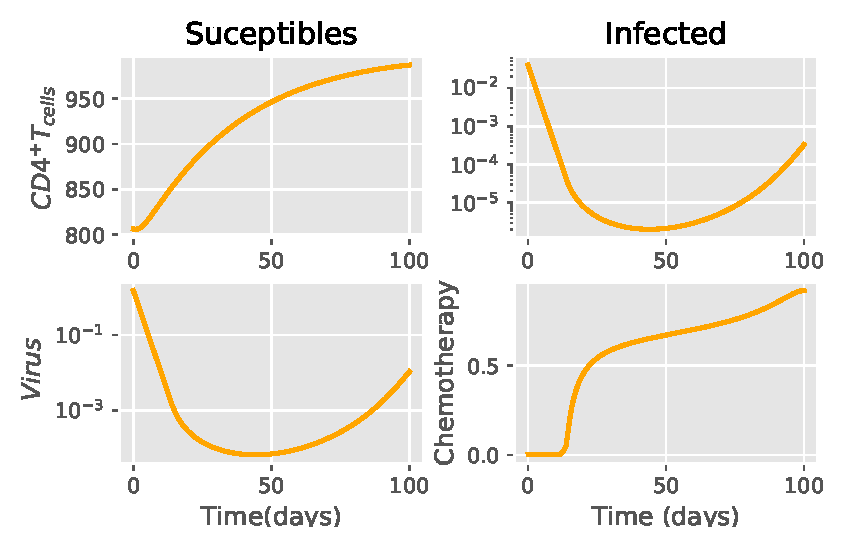
\includegraphics[width=0.7\linewidth]{Figures/hiv_chemotherapy_fig_01}
	\caption{Add description and stress the schedule of treatment}
	\label{fig:hivchemotherapyfig01}
\end{figure}

  \section{Case Finding and Case Control}
    \paragraph{Two-strains Tuberculosis Model.}
	Seeking to reduce the latent and infectious groups with the resistant-strain 
	tuberculosis, in \cite{Lenhart2002} the authors  use controls ro represents 
	two types of treatments in a tuberculosis model which consider the effect of 
	treatment in two kinds of strains. The uncontrolled version is:
	
	\begin{equation}\label{eqn:two_strain_TB}
	  \begin{aligned}
	    \frac{dS}{dt} &=
		    \Lambda - \beta_1 S \frac{I_1}{N} 
		    - \beta^{*} S \frac{I_2}{N}
		    - \mu S
		  \\
		  \frac{L_1}{dt} &=
			  \beta_1 S \frac{I_1}{N}
			  - (\mu + k_1) L_1
			  +  p r_2 I_1
				+ \beta_2 T \frac{I_1}{N}
				- \beta^{*} L_1 \frac{I_2}{N}
			\\
			\frac{I_1}{dt} &= 
				k_1 L_1
				- (\mu + d_1) I_1
				-r_2 I_1
			\\
			\frac{L_2}{dt} &=
				q r_2 I_1
				- (\mu + k_2) L_2
				+ \beta^{*} (S + L_1 + T) \frac{I_2}{N}
			\\
			\frac{I_2}{dt} &=
				k_2 L_2 - (\mu + d_2) I_2
			\\
			\frac{d T}{dt} &=
				r_1 L_1
				+ (1 - (p + q)) r_2 I_1
				- \beta T \frac{I_1}{N}
				- \beta^{*} T \frac{I_2}{N}
				-\mu T ~.
	  \end{aligned}
	\end{equation}

	\citeauthor*{Lenhart2002} consider time dependent 
optimal control strategies associated with case holding and case finding based 
% on the two-strain TB model \eqref{eqn:two_strain_TB}. They incorporates the 
case finding control by adding a term which identifies and cure a fraction o 
latent individuals. This control consequently reduces the rate of disease 
development by latent individuals. The authors includes case holding by adding a 
term which may decrease the treatment failure rate of individuals with sensitive 
TB, so,this control reduce the incidence of drug resistant TB. 

	Using $u_1(t)$ to denote the fraction of typical TB latent individuals that 
is identified and will put under treatment---case finding control--- and
$1 - u_2(t)$ to represent the effort that prevents the failure treatment in 
typical TB infectious individuals, the two-strain-TB model 
\eqref{eqn:two_strain_TB} becomes:
\begin{equation}
	  \begin{aligned}
	    \frac{dS}{dt} &=
		    \Lambda - \beta_1 S \frac{I_1}{N} 
		    - \beta^{*} S \frac{I_2}{N}
		    \mu S
		  \\
		  \frac{L_1}{dt} &=
			  \beta_1 S \frac{I_1}{N}
			  - (\mu + k_1) L_1
			  - u_1 (t) r_1 L_1
			  + (1 - u_2 (t)) p r_2 I_1
				+ \beta_2 T \frac{I_1}{N}
				- \beta^{*} L_1 \frac{I_2}{N}
			\\
			\frac{I_1}{dt} &= 
				k_1 L_1
				- (\mu + d_1) I_1
				-r_2 I_1
			\\
			\frac{L_2}{dt} &=
				(1 - u_2(t)) q r_2 I_1
				- (\mu + k_2) L_2
				+ \beta^{*} (S + L_1 + T) \frac{I_2}{N}
			\\
			\frac{I_2}{dt} &=
				k_2 L_2 - (\mu + d_2) I_2
			\\
			\frac{d T}{dt} &=
				u_1(t) r_1 L_1
				+ (1 - (1 - u_2(t))(p + q)) r_2 I_1
				- \beta T \frac{I_1}{N}
				- \beta^{*} T \frac{I_2}{N}
				-\mu T.
	  \end{aligned}
	\end{equation}

In this context, the controls reduce the latent and infected 
groups with resistant TB. However, case holding and case finding controls 
produces a economic fee. In \cite{Lenhart2002} the authors use
\begin{equation}
	 J(u_1, u_2) =
		 \int_0 ^ {t_f}
			 \left[
				 L_2(t) + I_2(t) 
				 + \frac{B_1}{2} [u_1(t)] ^ 2
				 + \frac{B_2}{2} [u_2(t)] ^ 2
			 \right]dt,
\end{equation}
to describe the regarding cost.
\begin{table}
	\begin{center}
		\begin{tabular}{@{}rll@{}} 
			$S:$
			&
				Susceptible
			\\
			$I:$ 
			&	Infected
			\\
			$R:$ 
			&	Recover
			\\
			\\
			%\toprule
			\multicolumn{1}{c}{Parameter}
			&
			\multicolumn{1}{c}{Meaning}
			& 
			\multicolumn{1}{c}{Value}
			\\
				\midrule
				$\beta$
				& 
					Transmission probability
				&
					---
			\\
				$\gamma$
				&
					Recover rate
			\\
				$\mu$
				&
					Natural death rate
			\\
				$K$
				&
					Carrying capacity
			\\
			\bottomrule
		\end{tabular}
		\caption{Variables and parameters description}
	\end{center}
\end{table}
  \section{Isolation and Quarantine}
    
\subsection*{SARS}
\citeauthor{Yan2008} report in \cite{Yan2008} a epidemic model for
Severe acute respiratory syndrome (SARS). They use quarantine and 
isolation as mitigation controls. The authors propose sub-optimal 
control policies and perform numeric simulations with genetic 
algorithms. The controlled version used in the mentioned 
reference reads:
%
%
\begin{equation}\label{eqn:sars_model}
	\begin{aligned}
		\dfrac{dS}{dt} &=
			\Lambda 
			-\dfrac{
				S
				\left(
					\beta I 
					+ \mathcal{E}_E  \beta E
					+ \mathcal{E}_Q  \beta Q
					+ \mathcal{E}_J  \beta J
				\right)
			}{N}
			- \mu S,
		\\
		\dfrac{dE}{dt} &=
			p +
			\dfrac{
				\beta S
				\left(
					\beta I 
						+ \mathcal{E}_E \beta E
						+ \mathcal{E}_Q \beta Q
						+ \mathcal{E}_J \beta J
				\right)
			}{N}
			-(
				u_1(t) + k_1 + \mu
			)E,
		\\
		\dfrac{dQ}{dt} &=
			u_1(t) E 
			- (k_2 + \mu) Q
		\\
		\dfrac{dI}{dt} &=
			k_1 E 
			-(u_2(t) + d_1  + \sigma_1 + \mu) I,
		\\
		\dfrac{dJ}{dt} &=
			u_2(t) I 
			+ k_2 Q
			- (d_2 + \sigma_2 + \mu) J,
		\\
		\dfrac{dR}{dt} &=
			\sigma_1 I
			+\sigma_2 J
			- \mu R.
	\end{aligned}
\end{equation}
The control variable $u_1$ denotes the proportion of quarantining people 
who had contact with an infected person inside of a quarantining program or
educational campaigns. Control $u_2$ models the proportion of symptomatic 
population which are in a isolation program. The authors consider the 
following epidemiological classes.
\begin{table}[h!]
	\begin{center}
		\begin{tabular}{@{}rll@{}} 
			$S$: & Susceptible individuals 
			\\
			$E$: & Asymptomatic individuals who have been 
			\\
			   & exposed to the virus but have not yet developed 
			\\
			   & clinical symptoms of SARS 
			\\
			$Q$: & Quarantine individuals
			\\
			$I$: & Symptomatic 
			\\
			$J$: & Isolated
			\\
			$R$: & Recovered
			\\
				& $N = S + E + Q + I + J + R$.
		\end{tabular}
	\end{center}
\end{table}
We enclose a description of the model parameters 
in \Cref{tbl:sars_table_des}.
So, giving the disease dynamics in \eqref{eqn:sars_model}, the problem is to 
minimize the functional cost
\begin{equation}\label{eqn:sars_cost}
  J(u_1,u_2)
    = \int_{0}^{t_f}
      \left[
        B_1 E(t)
        + B_2 Q(t)
        + B_3 I(t)
        + B_4 J(t)
        + \frac{C_1}{2} u_1^2 (t)
        + \frac{C_2}{2} u_2^2 (t)
      \right]
      dt.
\end{equation}
%
\begin{table}[H]
    \begin{center}
      \begin{tabular}{@{}rl@{}}
        \toprule
        & \multicolumn{1}{l}{\bf{Description}}
        \\
        \midrule
        $\beta$
          & Transmission coefficient
        \\
        $\varepsilon_E$, 
        $\varepsilon_Q$,
        $\varepsilon_J$
          & Modification parameter for 
          \\
          &  exposed, quarantine and isolation classes 
          \\
        $\mu$
          & Natural death rate.
        \\
        $\Lambda$
          & Constant recruitment rate
        \\
        $p$
          & Net inflow of asymptomatic individuals
        \\
        $k_1$ 
          & Transfer rate from class 
          \\
          & of asymptomatic to symptomatic
          \\
        $k_2$
          & Transfer rate from the quarantine 
          \\ 
          & class to isolation
        \\
        \\
        $d_1$, $d_2$
          & Per-capita disease induced death rates 
          \\
          & for the symptomatic individuals and 
          \\
          & isolated individuals.
        \\
        $\sigma_1$, $\sigma_2$
          & Per-capita recovery rates for the 
          \\
          & symptomatic individuals and 
          \\
          &  isolated individuals
        \\
        \\
        $t_f$
          & Final time 
        \\
        $B_1$, $B_2$, $B_3$, $B_4$
        & Respectively cost for 
        \\
        &
          $E$,$Q$,$I$,$J$ classes
        \\
        $C_1$, $C_2$
        & Costs for Isolation and Quarantine 
        \\
          & policies.
        \\
        \bottomrule
      \end{tabular}
     \caption{Parameter description for the SARS model
     \eqref{eqn:sars_model}.}
     \label{tbl:sars_table_des}
     \end{center}
\end{table}
  \section{Culling}
    Here we present the model reported in \cite*{Bolzoni2014} to describe a 
outbreak of bovine tuberculosis. The regarding uncontrolled model reads

\begin{equation}
	\begin{aligned}
  \min_{u(t)\in \mathcal{U}}
    &
    \int_0^T
      I(t) + P [u(t)]^{\theta}, \quad \theta \in \{1,2\},
      \quad P = B/A
  \\ \textrm{subject to:} &
  \\
    &\dfrac{dS}{dt} =
			r S 
			\left (
				1 - \dfrac{S+I}{K}
			\right)
			 - \beta SI - u(t) S
		\\
		&\dfrac{dI}{dt} =
			\beta SI - (\alpha + \mu + u(t)) I.
	\end{aligned}
\end{equation}
%

  \section{Existence and characterization of optimal policies}
  \section{Numerical analysis}
    \subsection{Popular methods}
\paragraph{Forward-Backward-Sweep}
\cite{hackbusch1978numerical}
\begin{algorithm}
	\caption{Forward Backward Sweep } \label{alg:forward_backward_sweep}
    \begin{flushleft}
    	\hspace*{\algorithmicindent} \textbf{Input:} 
    	$t_0, t_f, n_{max}, x_0,h, a, r, m, \epsilon, \lambda_{f}$ \\
    	\hspace*{\algorithmicindent} \textbf{Output:} 
   		$x^*, u^*, \lambda$
   	\end{flushleft}
	\begin{algorithmic}[1]
		\Procedure{Forward backward sweep}{$g,\lambda_{\text{function}}, 
        u, x_0, 
        \lambda_f, h, n_{max}$} 
			\While{$ \text{test} > \epsilon $}
				\State $u_{\text{old}} \gets u$ 
                \State $x_{\text{old}} \gets x$ 
                \State $ x \gets$
	                \Call{runge\_kutta\_forward}{$g, u, x_0, h$}
                \State $\lambda_{\text{old}} \gets \lambda $
				\State $\lambda \gets$ 
					\Call{runge\_kutta\_backward}{%
						$\lambda_{\text{function}}, x, \lambda_f, h$
					}
                \State $u_1 \gets$ 
                \Call{optimality\_condition}{$u, x, \lambda$}
                %
                \State 
                	$u \gets \alpha u_1 + (1-\alpha)u_{old}, 
                	\qquad \alpha \in [0, 1]$
                \Comment{convex combination}
                \State 
                	$\epsilon_u \gets \displaystyle 
                	\frac{||u - u_{\text{old}}||}{||u||}$
                \State 
                	$\epsilon_x \gets \displaystyle 
                	\frac{||x - x_{\text{old}}||}{||x||}$
                \Comment{relative error}
                \State 
                	$\epsilon_{\lambda} \gets \displaystyle 
                	\frac{||\lambda - \lambda_{\text{old}}||}{||\lambda||}$
                \State 
                	$\epsilon \gets 
                		\max{ 
                			\{ \epsilon_u, \epsilon_x, \epsilon_{\lambda} \}
                		}$
			\EndWhile\label{}
			\State \textbf{return} $ x^*, u^*, \lambda$
            \Comment{Optimal pair}
		\EndProcedure
	\end{algorithmic}
\end{algorithm}

  \section{Concluding remarks}
%
%
  \bibliographystyle{plainnat}
  \bibliography{references,OptimalControl-ContinuousControledEpidemicModels}
\end{document}